\chapter{Parte IV - Apresentações com o \textit{Beamer}}
\label{cap:parteIV}

\section{Pacote \textit{Beamer}}
\label{sec:beamer}

O \textit{Beamer} é o pacote padrão do \LaTeX{} para a produção de apresentações no estilo do \textit{Microsoft PowerPoint}. Assim como os documentos do \LaTeX{}, é possível reconhecer os documentos de apresentações produzidos pelo \textit{Beamer} pela sua qualidade gráfica e pelos seus estilos pré-definidos (embora seja possível criar estilos a partir do zero, esta tarefa não será abordada aqui).

Um documento do \textit{Beamer} é tão simples quanto um documento do \LaTeX{}. O {\tt beamer} é uma classe de documentos, essim como o {\tt article}, {\tt report}, {\tt book} etc. Para criar um documento \textit{Beamer}, basta utilizar esta classe. Veja no Exemplo \ref{exe:beamer1} a seguir, um exemplo mínimo.

\begin{texexptitled}[breakable,center lower,enhanced jigsaw,middle=2mm,listing side comment,righthand width=5.5cm,compilable listing,run latex,run dvips,run ps2pdf,pdf comment,comment style={raster columns=1},freeze pdf]{Um documento \textit{Beamer} mínimo}{exe:beamer1}
\documentclass{beamer}
\usepackage[utf8]{inputenc}
\usepackage{lipsum}

\title{Título}
\author{Nome}
\date{September 2019}

\begin{document}

\maketitle

\section{Seção}

\subsection{Subseção}

\begin{frame}{Frame}
\lipsum[1]
\end{frame}

\end{document}
\end{texexptitled}

Diferente de um documento \LaTeX{} mínimo, como aquele mostrado no Exemplo \ref{exe_doc}, um documento do \textit{Beamer} contém \textit{frames}, que são inseridos com o ambiente padrão {\tt frame}. Um \textit{frame} é um como um \textit{slide} do \textit{Microsoft PowerPoint} e dentro dele é possível inserir quaisquer ambientes que normalmente são inseridos dentro de um documento \LaTeX{} comum, e.g., listas, figuras, tabelas, texto, textos em colunas, ambientes especiais como o \textit{minipages}, \textit{listings} e outros.

Nas seções a seguir, são mostrados alguns detalhes de alguns dos elementos principais de um documento \textit{Beamer}.

\subsection{Estilos}
\label{sec:estilos}

Assim como qualquer outro editor de apresentações, no \textit{Beamer} também é possível utilizar temas e aplicar diferentes estilos e cores nas fontes e elementos da estrutura do documento. O estilo de um documento \textit{Beamer} pode ser definido através do tema, esquema de cores e estilo das fontes. Para isto, utiliza-se o comando \mintinline{latex}{\usetheme{tema}} no preâmbulo de um documento \textit{Beamer} de forma que seja definido um dos 28 temas padrão do \textit{Beamer}. Os nomes dos temas e os seus respectivos esquema de cores, são mostrados no Exemplo \ref{exe:beamer2} a seguir.

\begin{texexptitled}[breakable,center lower,enhanced jigsaw,text only]{Temas padrão do \textit{Beamer}}{exe:beamer2}
\begin{tcbitemize}[raster columns=3,bicolor,
raster equal height,boxrule=0.1mm,
colframe=MaterialGreen900,colback=MaterialGrey50,
pdf comment]
\tcbitem[squeezed title={default}]    \centering \includegraphics[scale=0.28,page=27]{./docs/figs/beamer.pdf}
\tcbitem[squeezed title={AnnArbor}]   \centering \includegraphics[scale=0.28,page=11]{./docs/figs/beamer.pdf}
\tcbitem[squeezed title={Antibes}]    \centering \includegraphics[scale=0.28,page=20]{./docs/figs/beamer.pdf}
\tcbitem[squeezed title={Bergen}]     \centering \includegraphics[scale=0.28,page=21]{./docs/figs/beamer.pdf}
\tcbitem[squeezed title={Berkeley}]   \centering \includegraphics[scale=0.28,page=22]{./docs/figs/beamer.pdf}
\tcbitem[squeezed title={Berlin}]     \centering \includegraphics[scale=0.28,page=23]{./docs/figs/beamer.pdf}
\tcbitem[squeezed title={Boadilla}]   \centering \includegraphics[scale=0.28,page=24]{./docs/figs/beamer.pdf}
\tcbitem[squeezed title={CambridgeUS}]\centering \includegraphics[scale=0.28,page=25]{./docs/figs/beamer.pdf}
\tcbitem[squeezed title={Copenhagen}] \centering \includegraphics[scale=0.28,page=26]{./docs/figs/beamer.pdf}
\tcbitem[squeezed title={Darmstadt}]  \centering 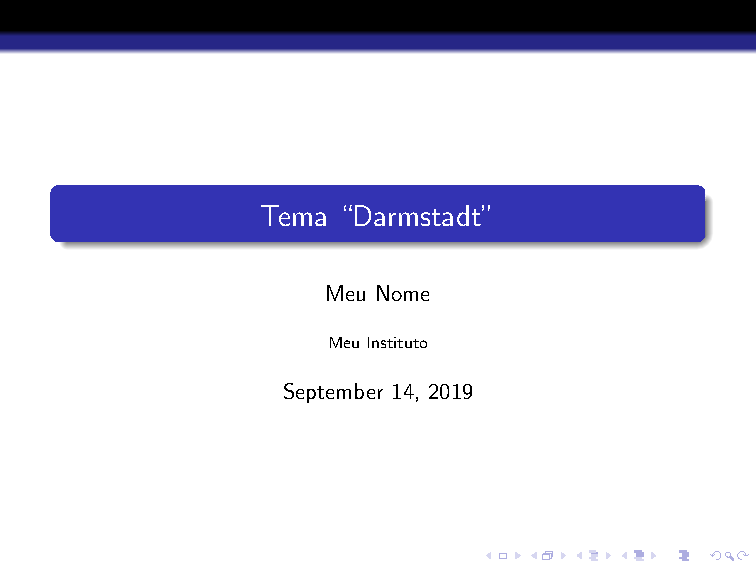
\includegraphics[scale=0.28,page=1] {./docs/figs/beamer.pdf}
\tcbitem[squeezed title={Dresden}]    \centering \includegraphics[scale=0.28,page=2] {./docs/figs/beamer.pdf}
\tcbitem[squeezed title={EastLansing}]\centering \includegraphics[scale=0.28,page=28]{./docs/figs/beamer.pdf}
\tcbitem[squeezed title={Frankfurt}]  \centering \includegraphics[scale=0.28,page=3] {./docs/figs/beamer.pdf}
\tcbitem[squeezed title={Goettingen}] \centering \includegraphics[scale=0.28,page=4] {./docs/figs/beamer.pdf}
\tcbitem[squeezed title={Hannover}]   \centering \includegraphics[scale=0.28,page=5] {./docs/figs/beamer.pdf}
\tcbitem[squeezed title={Ilmenau}]    \centering \includegraphics[scale=0.28,page=6] {./docs/figs/beamer.pdf}
\tcbitem[squeezed title={JuanLesPins}]\centering \includegraphics[scale=0.28,page=7] {./docs/figs/beamer.pdf}
\tcbitem[squeezed title={Luebeck}]    \centering \includegraphics[scale=0.28,page=8] {./docs/figs/beamer.pdf}
\tcbitem[squeezed title={Madrid}]     \centering \includegraphics[scale=0.28,page=9] {./docs/figs/beamer.pdf}
\tcbitem[squeezed title={Malmoe}]     \centering \includegraphics[scale=0.28,page=10]{./docs/figs/beamer.pdf}
\tcbitem[squeezed title={Marburg}]    \centering \includegraphics[scale=0.28,page=12]{./docs/figs/beamer.pdf}
\tcbitem[squeezed title={Montpellier}]\centering \includegraphics[scale=0.28,page=13]{./docs/figs/beamer.pdf}
\tcbitem[squeezed title={PaloAlto}]   \centering \includegraphics[scale=0.28,page=14]{./docs/figs/beamer.pdf}
\tcbitem[squeezed title={Pittsburg}]  \centering \includegraphics[scale=0.28,page=15]{./docs/figs/beamer.pdf}
\tcbitem[squeezed title={Rochester}]  \centering \includegraphics[scale=0.28,page=16]{./docs/figs/beamer.pdf}
\tcbitem[squeezed title={Singapore}]  \centering \includegraphics[scale=0.28,page=17]{./docs/figs/beamer.pdf}
\tcbitem[squeezed title={Szeged}]     \centering \includegraphics[scale=0.28,page=18]{./docs/figs/beamer.pdf}
\tcbitem[squeezed title={Warsaw}]     \centering \includegraphics[scale=0.28,page=19]{./docs/figs/beamer.pdf}
\end{tcbitemize}
\end{texexptitled}

Para cada um dos temas apresentados no Exemplo \ref{exe:beamer2}, é possível alterar o esquema de cores. Para isso, além de se utilizar o comando {\tt usetheme}, deve-se utilizar o comando \mintinline{latex}{\usecolortheme{esquema}}. Os esquemas de cores disponíveis para cada uma dos temas são os seguintes:

\begingroup
\renewcommand{\labelenumi}{\arabic{enumi})}
\begin{multicols}{3}
    \begin{enumerate}
      \item default
      \item albatross
      \item beaver
      \item beetle
      \item crane
      \item dolphin
      \item dove
      \item fly
      \item lily
      \item monarca
      \item orchid
      \item rose
      \item seagull
      \item seahorse
      \item spruce
      \item whale
      \item wolverine
    \end{enumerate}
\end{multicols}
\endgroup

No Exemplo \ref{exe:beamer2_tema} é mostrado o tema ``AnnArbor'' com o esquema de cores ``beaver''. Observe que este exemplo possui o mesmo código do Exemplo \ref{exe:beamer1}, com a diferença de que foram adicionados os comandos {\tt usetheme} e {\tt usecolortheme}.

\begin{texexptitled}[breakable,center lower,enhanced jigsaw,middle=2mm,listing side comment,righthand width=5.5cm,compilable listing,run latex,run dvips,run ps2pdf,pdf comment,comment style={raster columns=1},freeze pdf]{Um documento \textit{Beamer} mínimo com o tema ``AnnArbor'' e o esquema de cores ``beaver''}{exe:beamer2_tema}
\documentclass{beamer}
\usepackage[utf8]{inputenc}
\usepackage{lipsum}

\usetheme{AnnArbor}
\usecolortheme{beaver}

\title{Título}
\author{Nome}
\date{September 2019}

\begin{document}

\maketitle

\begin{frame}{Frame}
\lipsum[1]
\end{frame}

\end{document}
\end{texexptitled}

\begin{marker}
Veja mais opções de temas e as variações dos esquemas de cores do \textit{Beamer} em \url{https://hartwork.org/beamer-theme-matrix/}.
\end{marker}

Além da escolha do tema e do esquema de cores, é possível também alterar as cores e estilos de fontes de diferentes elementos visuais dos temas, de forma individual. O comando \mintinline{latex}{\setbeamercolor{tema}{elemento(s)}} define o esquema de cores que será utilizado e quais elementos do tema escolhido deverão ser alterados. O comando \mintinline{latex}{\setbeamerfont{tema}{elemento(s)}}, da mesma forma, permite alterar o estilo das fontes do tema escolhido. São muitos os elementos que podem ser alterados dentro de um \textit{frame} do \textit{Beamer} e, portanto, a apresentação deles foge ao escopo deste material.

\begin{marker}
Para conhecer mais sobre as possibilidades de customização dos diversos elementos de um \textit{frame} do \textit{Beamer}, recomenda-se a leitura da documentação do pacote em \url{http://linorg.usp.br/CTAN/macros/latex/contrib/beamer/doc/beameruserguide.pdf}.
\end{marker}

\subsection{Ambientes especiais}
\label{sec:estrut_slide}

Em um \textit{frame} do \textit{Beamer}, podem ser inseridas listas, tabelas, imagens, equações e outros ambientes que já foram mostrados no Capítulo \ref{cap:parteII}. Além destes ambientes, o \textit{Beamer} suporta também ambientes especiais que podem ser utilizados para destacar as informações inseridas. Um destes ambientes especiais, é o ambiente \mintinline{latex}{block}. Veja no Exemplo \ref{exe:beamer_block} a seguir como inserí-lo em um \textit{frame} do \textit{Beamer}:

\begin{texexptitled}[breakable,center lower,enhanced jigsaw,middle=2mm,listing side comment,righthand width=5.5cm,compilable listing,run latex,run dvips,run ps2pdf,pdf comment,comment style={raster columns=1},freeze pdf]{Ambiente {\tt block} em um \textit{frame} do \textit{Beamer}}{exe:beamer_block}
\documentclass{beamer}
\usepackage[utf8]{inputenc}

\usetheme{Bergen}

\title{Título}
\author{Nome}
\date{September 2019}

\begin{document}

\maketitle

\begin{frame}{Meu Frame}
  \begin{block}{Meu block}
    À noite, vovô Kowalsky vê o ímã cair no pé do pinguim queixoso e vovó põe açúcar no chá de tâmaras do jabuti feliz. 
  \end{block}
\end{frame}

\end{document}
\end{texexptitled}

Além do ambiente {\tt block}, há também os ambientes {\tt exampleblock} e {\tt alertblock}. Cada um deles pode ser utilizado em situações distintas, dando importância ou chamando a atenção para determinadas partes da apresentação. Veja no Exemplo \ref{exe:beamer_blocks} a seguir, um exemplo do uso destes ambientes.

\begin{texexptitled}[breakable,center lower,enhanced jigsaw,middle=2mm,listing side comment,righthand width=5.5cm,compilable listing,run latex,run dvips,run ps2pdf,pdf comment,comment style={raster columns=1},freeze pdf]{Ambiente {\tt block} em um \textit{frame} do \textit{Beamer}}{exe:beamer_blocks}
\documentclass{beamer}
\usepackage[utf8]{inputenc}

\usetheme{Warsaw}

\title{Título}
\author{Nome}
\date{September 2019}

\begin{document}

\maketitle

\begin{frame}{Meu fFrame}
  \begin{block}{Bloco {\tt block}}
    À noite, vovô Kowalsky vê o ímã cair no pé do pinguim queixoso e vovó põe açúcar no chá de tâmaras do jabuti feliz. 
  \end{block}
  \begin{exampleblock}{Bloco {\tt exampleblock}}
    Quem traz CD, LP, fax, engov e whisky JB?
  \end{exampleblock}
  \begin{alertblock}{Bloco {\tt alertblock}}
    Jane quer LP, fax, CD, giz, TV e bom whisky.
  \end{alertblock}
\end{frame}

\end{document}
\end{texexptitled}

\subsection{Informações da Capa}
\label{sec:info_capa}

Como em toda apresentação, é comum o primeiro \textit{frame} ou \textit{slide} possuir informações como título (\mintinline{latex}{\title{}}), subtítulo (\mintinline{latex}{\subtitle{}}), autor (\mintinline{latex}{\author{}}), afiliação (\mintinline{latex}{\institute{}}), data (\mintinline{latex}{\date{}}), local e, eventualmente, alguma figura com o logo do evento ou da instituição (\mintinline{latex}{\titlegraphic{}}). O Exemplo \ref{exe:beamer_capa1} mostra o uso destas macros para incluir as informações mais comuns na capa de uma apresentação confeccionada com o \textit{Beamer}. %No \textit{Beamer}, estas informações podem ser inseridas a partir das \textit{macros} a seguir:

%\begin{itemize}
%  \begin{itemize}
%    \item Título: \mintinline{latex}{\title{}};
%    \item Subtítulo: \mintinline{latex}{\subtitle{}};
%    \item Autor: \mintinline{latex}{\author{}};
%    \item Afiliação: \mintinline{latex}{\institute{}};
%    \item Data: \mintinline{latex}{\date{}};
%    \item Logo: \mintinline{latex}{\titlegraphic{}};
%  \end{itemize}
%\end{itemize}

%O Exemplo \ref{exe:beamer_capa1} mostra o uso destas macros para incluir as informações mais comuns na capa de uma apresentação confeccionada com o \textit{Beamer}.

\begin{texexptitled}[enhanced jigsaw, lower separated=true, leftlower=0pt,rightlower=0pt,listing and comment,compilable listing,run latex,run dvips,run ps2pdf,pdf comment,comment style={raster columns=1},freeze pdf]{Informações da Capa em uma apresentação do \textit{Beamer}}{exe:beamer_capa1}
\documentclass{beamer}
\usepackage[utf8]{inputenc}

\usetheme{Luebeck}

\title{Título}
\subtitle{Subtítulo}
\author{Nome}
\institute{Meu Instituto}
\date{September 2019}

\titlegraphic{
\includegraphics[scale=0.25]{docs/figs/logo.eps}}

\begin{document}

\maketitle

\end{document}
\end{texexptitled}

Caso seja do interesse do usuário, este poderá manter a data sempre atualizada a partir da utilização da \textit{macro} \mintinline{latex}{\today}, que sempre irá incorpoerar a data do dia em que a apresentação foi compilada. Logo, ao invés de inserir \mintinline{latex}{\date{September 2019}}, insira \mintinline{latex}{\date{\today}}.

\subsection{Sumário}
\label{sec:bsumario}

Assim como em documentos \LaTeX{}, as apresentações escritas com a classe \textit{Beamer} também podem conter um sumário com as seções e subseções. No Exemplo \ref{exe:beamer1}, o código inclui uma seção e uma subseção e os \textit{frames} da apresentação podem ser organizados utilizando estas partições. Para inserir um sumário em uma apresentação \textit{Beamer}, basta inserir a \textit{macro} \mintinline{latex}{\tableofcontents}\footnote{Quando o sumário é adicionado ao documento \textit{Beamer}, pode ser necessário compilar o documento mais de uma vez.} no primeiro \textit{frame} da apresentação. O Exemplo \ref{exe:beamer_sumario1} mostra como inserir um Sumário na apresentação \textit{Beamer}.

\begin{texexptitled}[breakable,center lower,enhanced jigsaw,middle=2mm,listing side comment,righthand width=5.5cm,compilable listing,run latex,run dvips,run ps2pdf,pdf comment,comment style={raster columns=1},freeze pdf]{Sumário em um documento \textit{Beamer}}{exe:beamer_sumario1}
\documentclass{beamer}
\usepackage[utf8]{inputenc}
\usepackage{lipsum}

\usetheme{Madrid}

\title{Título}
\author{Nome}
\date{September 2019}

\begin{document}

\maketitle

\begin{frame}[c]{Sumário}
\tableofcontents
\end{frame}

\section{Uma Seção}

\subsection{Uma Subseção}

\begin{frame}{Frame 1}
  \lipsum[1]
\end{frame}

\end{document}
\end{texexptitled}

Dependendo da forma como a apresentação é organizada, e dependendo também do tema escolhido, pode ser conveniente alterar a aparência ou o comportamento do sumário. Isto significa que é possível omitir alguns elementos (e.g., subseções) do sumário ou mesmo fazer com que ele se repita toda vez que uma nova seção da apresentação é iniciada. Veja no Exemplo \ref{exe:beamer_sumario2} como omitir as subseções do sumário, utilizando uma opção {\tt hideallsubsections} da \textit{macro} \mintinline{latex}{\tableofcontents}.

\begin{texexptitled}[breakable,center lower,enhanced jigsaw,middle=2mm,listing side comment,righthand width=5.5cm,compilable listing,run latex,run dvips,run ps2pdf,pdf comment,comment style={raster columns=1},freeze pdf]{Sumário em um documento \textit{Beamer}, omitindo as subseções}{exe:beamer_sumario2}
\documentclass{beamer}
\usepackage[utf8]{inputenc}
\usepackage{lipsum}

\usetheme{Singapore}

\title{Título}
\author{Nome}
\date{September 2019}

\begin{document}

\maketitle

\begin{frame}[c]{Sumário}
\tableofcontents[hideallsubsections]
\end{frame}

\section{Uma Seção}

\subsection{Uma Subseção}

\begin{frame}{Frame 1}
  \lipsum[1]
\end{frame}

\end{document}
\end{texexptitled}

Para alterar o comportamento do sumário em um documento \textit{Beamer}, de forma que ele apareça sempre que uma nova seção for iniciada, pode-se incluir um novo \textit{frame} logo após o início da seção, incluindo a \textit{macro} \mintinline{latex}{\tableofcontents} com a opção {\tt currentsection} e/ou a opção {\tt currentsubsection}. Veja no Exemplo \ref{exe:beamer_sumario3} a seguir:

\begin{texexptitled}[breakable,center lower,enhanced jigsaw,middle=2mm,listing side comment,righthand width=5.5cm,compilable listing,run latex,run dvips,run ps2pdf,pdf comment,comment style={raster columns=1},freeze pdf]{Alterando o comportamento do sumário em um documento \textit{Beamer}}{exe:beamer_sumario3}
\documentclass{beamer}
\usepackage[utf8]{inputenc}
\usepackage{lipsum}

\usetheme{Szeged}

\title{Título}
\author{Nome}
\date{September 2019}

\begin{document}

\begin{frame}[c]{Sumário}
  \tableofcontents
\end{frame}

\section{Uma Seção}

\subsection{Uma Subseção}

\begin{frame}{Sumário}
  \tableofcontents[currentsection]
\end{frame}

\begin{frame}{Frame 1}
  \lipsum[1]
\end{frame}

\section{Uma Outra Seção}

\subsection{Uma Outra Subseção}

\begin{frame}[c]{Sumário}
  \tableofcontents[currentsection]
\end{frame}

\begin{frame}{Frame 2}
  \lipsum[2]
\end{frame}

\end{document}
\end{texexptitled}

\subsection{Barra de Navegação}
\label{sec:navbar}

Outro elemento que aparece na capa (e também dos demais \textit{frames}), é a barra de navegação. Essa barra serve para facilitar a navegação entre os \textit{slides} da apresentação, mas requer a utilização do \textit{mouse}, o que pode não ser muito prático. Nos temas pré-definidos do \textit{Beamer}, há uma barra de navegação persistente que é mostrada em detalhes na Figura \ref{fig:navbar}:

\begin{figure}[H]
\caption{A barra de navegação do \textit{Beamer}.}
\vspace{6mm}
  \begin{center}
    
\includegraphics[trim={8cm 0.35cm 0 8.75cm}, clip, scale=3]{./docs/figs/beamer-capa.pdf}
  \end{center}
\vspace{4mm}
\legenda{A barra de navegação do \textit{Beamer} sempre aparece em uso com os temas padrão do \textit{Beamer}. Entretanto, é possível desabilitá-la.}
\label{fig:navbar}
\FONTE{Produção do autor.}
\end{figure}

Para desabilitar a barra de navegação, basta utilizar um dos comandos a seguir: \mintinline{latex}{\beamertemplatenavigationsymbolsempty} ou \mintinline{latex}{\setbeamertemplate{navigation symbols}{}}.

Veja no Exemplo \ref{exe:navbar} a seguir o efeito do uso de um destes comandos:

\begin{texexptitled}[breakable,center lower,enhanced jigsaw,middle=2mm,listing side comment,righthand width=5.5cm,compilable listing,run latex,run dvips,run ps2pdf,pdf comment,comment style={raster columns=1},freeze pdf]{Desabilitando a barra de navegação do \textit{Beamer}}{exe:navbar}
\documentclass{beamer}
\usepackage[utf8]{inputenc}

\usepackage{lipsum}

\usetheme{PaloAlto}

\beamertemplatenavigationsymbolsempty

\title{Título}
\author{Nome}
\date{September 2019}

\begin{document}

\maketitle

\begin{frame}{Meu frame}

\lipsum[1]

\end{frame}

\end{document}
\end{texexptitled}

%\subsection{Numeração dos \textit{frames}}
%\label{sec:framenum}
%
%Os \textit{frames} do \textit{Beamer} podem ser numerados utilizando algumas \textit{macros} especiais que alteram o \textit{template} do tema escolhido. Alguns temas possuem um rodapé diferente do outro (de fato, alguns possuem, e outros não). Logo, a forma de introduzir a numeração dos \textit{frames} pode variar e, de forma geral, o usuário pode experimentar incluir o seguinte comando no preâmbulo do seu documento \textit{Beamer}: \mintinline{latex}{\setbeamertemplate{caption}[numbered]}. 
%
%\begin{texexptitled}[breakable,center lower,enhanced jigsaw,middle=2mm,listing side comment,righthand width=5.5cm,compilable listing,run latex,run dvips,run ps2pdf,pdf comment,comment style={raster columns=1},freeze pdf]{Controlando itens em uma lista no \textit{Beamer} com o comando {\tt onslide}}{exe:beamer_numeracao}
%\documentclass{beamer}
%\usepackage[utf8]{inputenc}
%
%\usetheme{Singapore}
%\beamertemplatenavigationsymbolsempty
%\setbeamertemplate{caption}[numbered]
%
%\title{Título}
%\author{Nome}
%\date{September 2019}
%
%\begin{document}
%
%\begin{frame}{Meu Frame}
%Minha lista:
%\onslide<1->
%\begin{enumerate}
%  \item\onslide<3> Item 1
%  \item\onslide<2-> Item 2
%  \item\onslide<4-> Item 3
%\end{enumerate}
%\onslide<2> Uma frase
%\end{frame}
%
%\end{document}
%\end{texexptitled}

\subsection{Transições e Animações}
\label{sec:trans_anima}

Efeitos de transição e animações também podem ser utilizadas em um documento \textit{Beamer}. Entretanto, observe que, diferentemente do \textit{Microsoft PowerPoint}, estes efeitos e animações são como as animações feitas em \textit{flipboards}, i.e., animações quadro-a-quadro. Isso significa que vários \textit{frames} (ou \textit{slides}) são produzidos até que a animação ou o efeito final seja alcançado. Veja no Exemplo \ref{exe:beamer3} como os itens de uma lista são apresentados de forma que apenas o item atual esteja realçado. Este efeito é muito comum e recebe o nome de pausa e ele é obtido a partir do comando \mintinline{latex}{\pause}.

% Ref. dos exemplos: http://web.mit.edu/rsi/www/pdfs/beamer-tutorial.pdf

\begin{texexptitled}[breakable,center lower,enhanced jigsaw,middle=2mm,listing side comment,righthand width=5.5cm,compilable listing,run latex,run dvips,run ps2pdf,pdf comment,comment style={raster columns=1},freeze pdf]{Adicionando pausas no \textit{Beamer} com o comando {\tt pause}}{exe:beamer3}
\documentclass{beamer}
\usepackage[utf8]{inputenc}

\usetheme{CambridgeUS}

\title{Título}
\author{Nome}
\date{September 2019}

\begin{document}

\maketitle

\begin{frame}{Meu Frame}
Minha Lista:
\begin{itemize}
    \pause
    \item Item 1
    \pause
    \item Item 2
    \pause
    \item Item 3
\end{itemize}
\end{frame}

\end{document}
\end{texexptitled}

Observe no Exemplo \ref{exe:beamer3} que os itens da lista são adicionados um após o outro de forma sequencial. Este comportamento pode ser alterado de forma que a ordem em que os itens aparecem possa ser controlada. Compare o Exemplo \ref{exe:beamer3} com o Exemplo \ref{exe:beamer4} a seguir:

\begin{texexptitled}[breakable,center lower,enhanced jigsaw,middle=2mm,listing side comment,righthand width=5.5cm,compilable listing,run latex,run dvips,run ps2pdf,pdf comment,comment style={raster columns=1},freeze pdf]{Controlando itens em uma lista no \textit{Beamer}}{exe:beamer4}
\documentclass{beamer}
\usepackage[utf8]{inputenc}

\usetheme{EastLansing}

\title{Título}
\author{Nome}
\date{September 2019}

\begin{document}

\maketitle

\begin{frame}{Meu Frame}
Minha Lista:
\pause
\begin{itemize}
    \item<2-> Item 1
    \item<3-> Item 2
    \item<4-> Item 3
\end{itemize}
\end{frame}

\end{document}
\end{texexptitled}

No Exemplo \ref{exe:beamer4}, não foi utilizado o comando \mintinline{latex}{\pause} e, ao invés dele, foram adicionados parâmetros ao comando \mintinline{latex}{\item} de forma que fosse especificado em qual \textit{slide} aquela informação da lista deve aparecer. Dessa forma, o comando \mintinline{latex}{\item<2-> Item 1} deve aparecer apenas no \textit{slide} número 2, o item descrito pelo comando \mintinline{latex}{\item<3-> Item 2} deve aparecer apenas no slide número 3 e assim por diante. Além disso, observe que há um sinal de {\tt -} (menos) após o número do \textit{slide}, indicando que aquele item irá aparecer a partir do número do \textit{slide} indicado em diante. Na Tabela \ref{tab:beamer1} estão listados alguns dos comandos de controle dos elementos de um \textit{slide} do \textit{Beamer}.

\begin{table}[H]
\centering
\caption{Alguns comandos de controle dos elementos de um \textit{slide} do \textit{Beamer}.}
\label{tab:beamer1}
    \begin{tabular}{p{2.5cm}p{8.5cm}}
    \toprule
    \textbf{Comando} & \textbf{Descrição} \\
    \midrule
    \mintinline{latex}{\textbf<>{}} & Controla quando um texto deverá ocorrer em negrito \\
    \mintinline{latex}{\textit<>{}} & Controle quando um texto deverá ocorrer em itálico \\
    \mintinline{latex}{\color<>{}} & Controla quando um texto deverá ocorrer em uma cor diferente \\
    \mintinline{latex}{\alert<>{}} & Controla quando um texto deverá ocorrer destacadamente \\
    \bottomrule
    \end{tabular}
\FONTE{Produção do autor.}
\end{table}

Outra \textit{macro} do \textit{Beamer} que permite controlar as ações dos efeitos de pausa e transição, é o \mintinline{latex}{\onslide}. Este comando permite indicar em qual \textit{slide} um determinado item deverá ocorrer. Veja no Exemplo \ref{exe:beamer_onslide} o seu funcionamento. No exemplo, observe que a capa da apresentação foi suprimida com a exclusão da \textit{maxcro} {\tt maketitle}, Além disso, note quando os itens e elementos permanecem ou não nos \textit{frames} produzidos.

\begin{texexptitled}[breakable,center lower,enhanced jigsaw,middle=2mm,listing side comment,righthand width=5.5cm,compilable listing,run latex,run dvips,run ps2pdf,pdf comment,comment style={raster columns=1},freeze pdf]{Controlando itens em uma lista no \textit{Beamer} com o comando {\tt onslide}}{exe:beamer_onslide}
\documentclass{beamer}
\usepackage[utf8]{inputenc}

\usetheme{Marburg}

\title{Título}
\author{Nome}
\date{September 2019}

\begin{document}

\begin{frame}{Meu Frame}
Minha lista:
\onslide<1->
\begin{enumerate}
  \item\onslide<3> Item 1
  \item\onslide<2-> Item 2
  \item\onslide<4-> Item 3
\end{enumerate}
\onslide<2> Uma frase
\end{frame}

\end{document}
\end{texexptitled}

\begin{marker}
No \LaTeX{} há outros pacotes que também podem ser utilizados para a confecção de apresentações e pôsteres no estilo do \textit{Microsoft PowerPoint}. Entre eles, destacam-se a classe {\tt powerdot} (\url{https://www.ctan.org/pkg/powerdot}) que fornece estilos muito semelhantes àqueles que podem ser encontrados no \textit{Microsoft PowerPoint} e o pacote {\tt tcolorbox} (\url{https://www.ctan.org/pkg/tcolorbox}).
\end{marker}
